\section{Methodik}
Dieses Kapitel beschreibt die Methodik der Arbeit. Zunächst wird die verwendete Datenbasis erläutert
und die Datenbeschaffung beschrieben. Anschließend wird die verwendete Methode zur Berechnung der
kürzesten Wege vorgestellt.

\subsection{Datenbeschaffung und -aufbereitung}

\subsection{Datenformat}
Das \ac{OSM}-Datenformat ist ein XML-basiertes Format, das aus drei verschiedenen Elementen besteht:
\begin{itemize}
    \item Knoten (Nodes): Knoten repräsentieren einzelne Punkte im Raum und werden durch ihre
          Längen- und Breitengrade (Geokoordinaten) definiert. Sie können Attribute wie Tags
          (Schlüssel-Wert-Paare) enthalten, um Sachdaten über den Punkt zu speichern, \zB den
          Namen, die Art des Ortes oder andere Eigenschaften.

    \item Wege (Ways): Wege bestehen aus einer geordneten Liste von Knoten und repräsentieren
          Linienzüge. In der Regel werden Straßen, Flüsse und Grenzen als Wege dargestellt. Wege
          können auch Tags enthalten, um zusätzliche Informationen über den Linienzug zu speichern,
          z. B. den Straßentyp oder die Geschwindigkeitsbegrenzung.

    \item Relationen (Relations): Relationen bestehen aus ein oder mehreren Attributen und einer
          sortierten Liste von Datenelementen (Wege, Knoten, Relationen), wobei  jedem Datenelement
          eine Rolle zugewiesen wird. Sie werden verwendet, um logische oder geometrische
          Zusammenhänge zwischen anderen Elementen zu beschreiben.
\end{itemize}
Grundsätzlich können beliebige Tags gesetzt werden, es haben sich jedoch zwei Arten von Tags
etabliert:

\emph{Klassifizierende} Tags haben einen von wenigen Schlüsseln, für jeden der wenigen Schlüssel
gibt es nur eine begrenzte Anzahl von Werten. Abweichende Werte werden als Fehler betrachtet. So
wird das gesamte öffentliche Straßennetz für Kraftfahrzeuge mit dem Schlüssel \emph{highway} und
einem von wenigen gemeinsamen Werten identifiziert. Für Gebäude ist in den meisten Fällen nur
\emph{building} mit dem Wert \emph{yes} definiert.

Im Gegensatz dazu haben die \emph{beschreibenden} Tags nur feste Schlüssel, während der Wert ein
freier Text ist, der in Groß- und Kleinbuchstaben geschrieben werden kann und auch Sonderzeichen
enthalten kann. Der Hauptanwendungsfall sind Namen. Dazu können Beschreibungen, Bezeichner oder auch
Größenangaben kommen.

Für diese Arbeit sind vorallem die Elemente \emph{Node} und \emph{Way} relevant, sowie der Tag
\emph{highway}. Abbildung~\ref{fig:osm_xml} zeigt ein Beispiel eines OSM-Dokuments. Es enthält drei
Knoten und einen Weg. Der Weg referenziert die drei Knoten über die \texttt{ref}-Attribute. Die
Straße ist vom Typ "`residential"', also eine Straße für Anlieger. Die weiteren Tags geben
außerdem die Information, dass die Straße eine Einbahnstraße ist und dass maximal 30 km/h
erlaubt sind.

\begin{figure}[h]
    % \begin{lstlisting}[language=xml, caption=Hello World in Java, captionpos=b]
    \begin{lstlisting}[language=xml]
<?xml version="1.0" encoding="UTF-8"?>
<osm version="0.6" upload="true" generator="OpenStreetMap server">
  <bounds minlat="51.5073601795557" minlon="-0.108157396316528" maxlat="51.5076406454029" maxlon="-0.107599496841431"/>
  <node id="1" lat="51.5074089" lon="-0.1080108" timestamp="1970-01-01T00:00:01Z" user="matt" visible="true" version="1"/>
  <node id="2" lat="51.5074343" lon="-0.1080123" timestamp="1970-01-01T00:00:01Z" user="snsn1" visible="true" version="1"/>
  <node id="3" lat="51.5075933" lon="-0.1076109" timestamp="1970-01-01T00:00:01Z" user="snsn1" visible="true" version="1"/>
  <way id="12" action="modify" timestamp="1970-01-01T00:00:01Z" visible="true" version="3">
    <nd ref="1" />
    <nd ref="2" />
    <nd ref="3" />
    <tag k="highway" v="residential" />
    <tag k="oneway" v="false" /> 
    <tag k="maxspeed" v="30"/>
    <tag k="name" v="Amselweg"/>
  </way>
</osm>
\end{lstlisting}
    \caption[OSM-XML-Beispiel]{Beispiel eines OSM-XML-Dokuments. Es enthält drei Knoten und einen
        Weg. Hierbei handelt es sich um eine Anliegerstraße (erkennbar am
        Tag \texttt{highway=residential}) mit erlaubter Höchstgeschwindigkeit von 30 km/h.}
    \label{fig:osm_xml}
\end{figure}

Es gibt keine klaren Vorgaben zum Taggen von Objekten nur Empfehlungen. Daher ist eine große
Variation an Tags zu erwarten, die ensprechend behandelt werden müssen.


\subsubsection{Datenextraktion}
Die erste Aufgabe besteht darin, die relevanten Daten aus dem OpenStreetMap-Datensatz zu
extrahieren. Hierzu gibt es zahlreiche Möglichkeiten und Werkzeuge. Die Geofabrik GmbH Karlsruhe
(Mitglied der \ac{OSM}-Foundation) bietet \ua ein Service an, bei dem sich bereits vorgefertigte
Regionen (hierarchisch unterteilt in Kontinente, Länder, Bundesländer, etc.) direkt herunterladen
lassen. Die Datensätze werden in der Regel täglich aktualisiert und sind als OSM- oder
PBF-Format\footnote{PBF: ("`Protocolbuffer Binary Format"') ist eine Alternative zum XML Format, die
    OSM-Rohdaten speichereffizient in Blöcken abspeichert \cite{osm.pbf}).} verfügbar
\cite{osm.geofabrik}.

Eine weitere Möglichkeit ist die Verwendung von \acp{API} wie \zB der
Overpass-\ac{API}\footnote{\url{https://overpass-api.de/}}, eine kostenlose Schnittstelle mit der
sich gezielt \ac{OSM}-Daten extrahieren lassen. Die Abfragen werden in der Overpass Query Language
(kurz: Overpass QL) erstellt, mit der sich Daten \ua nach bestimmten Tags filtern lassen, \zB nach
bestimmten Straßentypen oder Straßennamen \cite{osm.overpass}.

Beide Ansätze können verwendet werden, in der Arbeit werden aber hauptsächlich vorgefertigte Daten
im PBF-Format verwendet und verarbeitet. Zur Untersuchung von kleinen Gebieten wird die
Pyhtonbibliothek \emph{OSMNX} verwendet, die es ermöglicht, \ac{OSM}-Daten über eine
Highlevel-\ac{API} (intern: Overpass) abzufragen, zu verarbeiten und zu visualisieren.

\subsubsection{Datenverarbeitung}

\subsection{Contraction Hierarchies}
\subsubsection{Überblick}
Straßennetzwerke weisen eine sehr hierarchische Struktur auf. Es gibt "`wichtigere"' Straßen wie \zB
Autobahnen und "`unwichtigere"' Straßen wie \zB Straßen in Wohnsiedlungen (siehe
Abbildung~\ref{fig:road_hierarchy}). Um von einem entfernten Ort zu einem anderen zu gelangen, ist
es daher nur sinvoll, sich über Straßen mit zunehmender Wichtigkeit zu bewegen. Bei einer Suche
könnte die Information des Straßentyps und der damit verbundenen Wichtigkeit als Heuristik verwendet
werden, um bestimmte Kanten, die auf weniger wichtige Straßen führen,  zu ignorieren und damit die
Suche zu beschleunigen. Das Problem hierbei ist allerding, dass mit dieser Methode keine Garantie
besteht, dass der gefundene Weg auch wirklich der \emph{exakt} kürzeste Weg ist.
\begin{figure}[h]
    \centering
    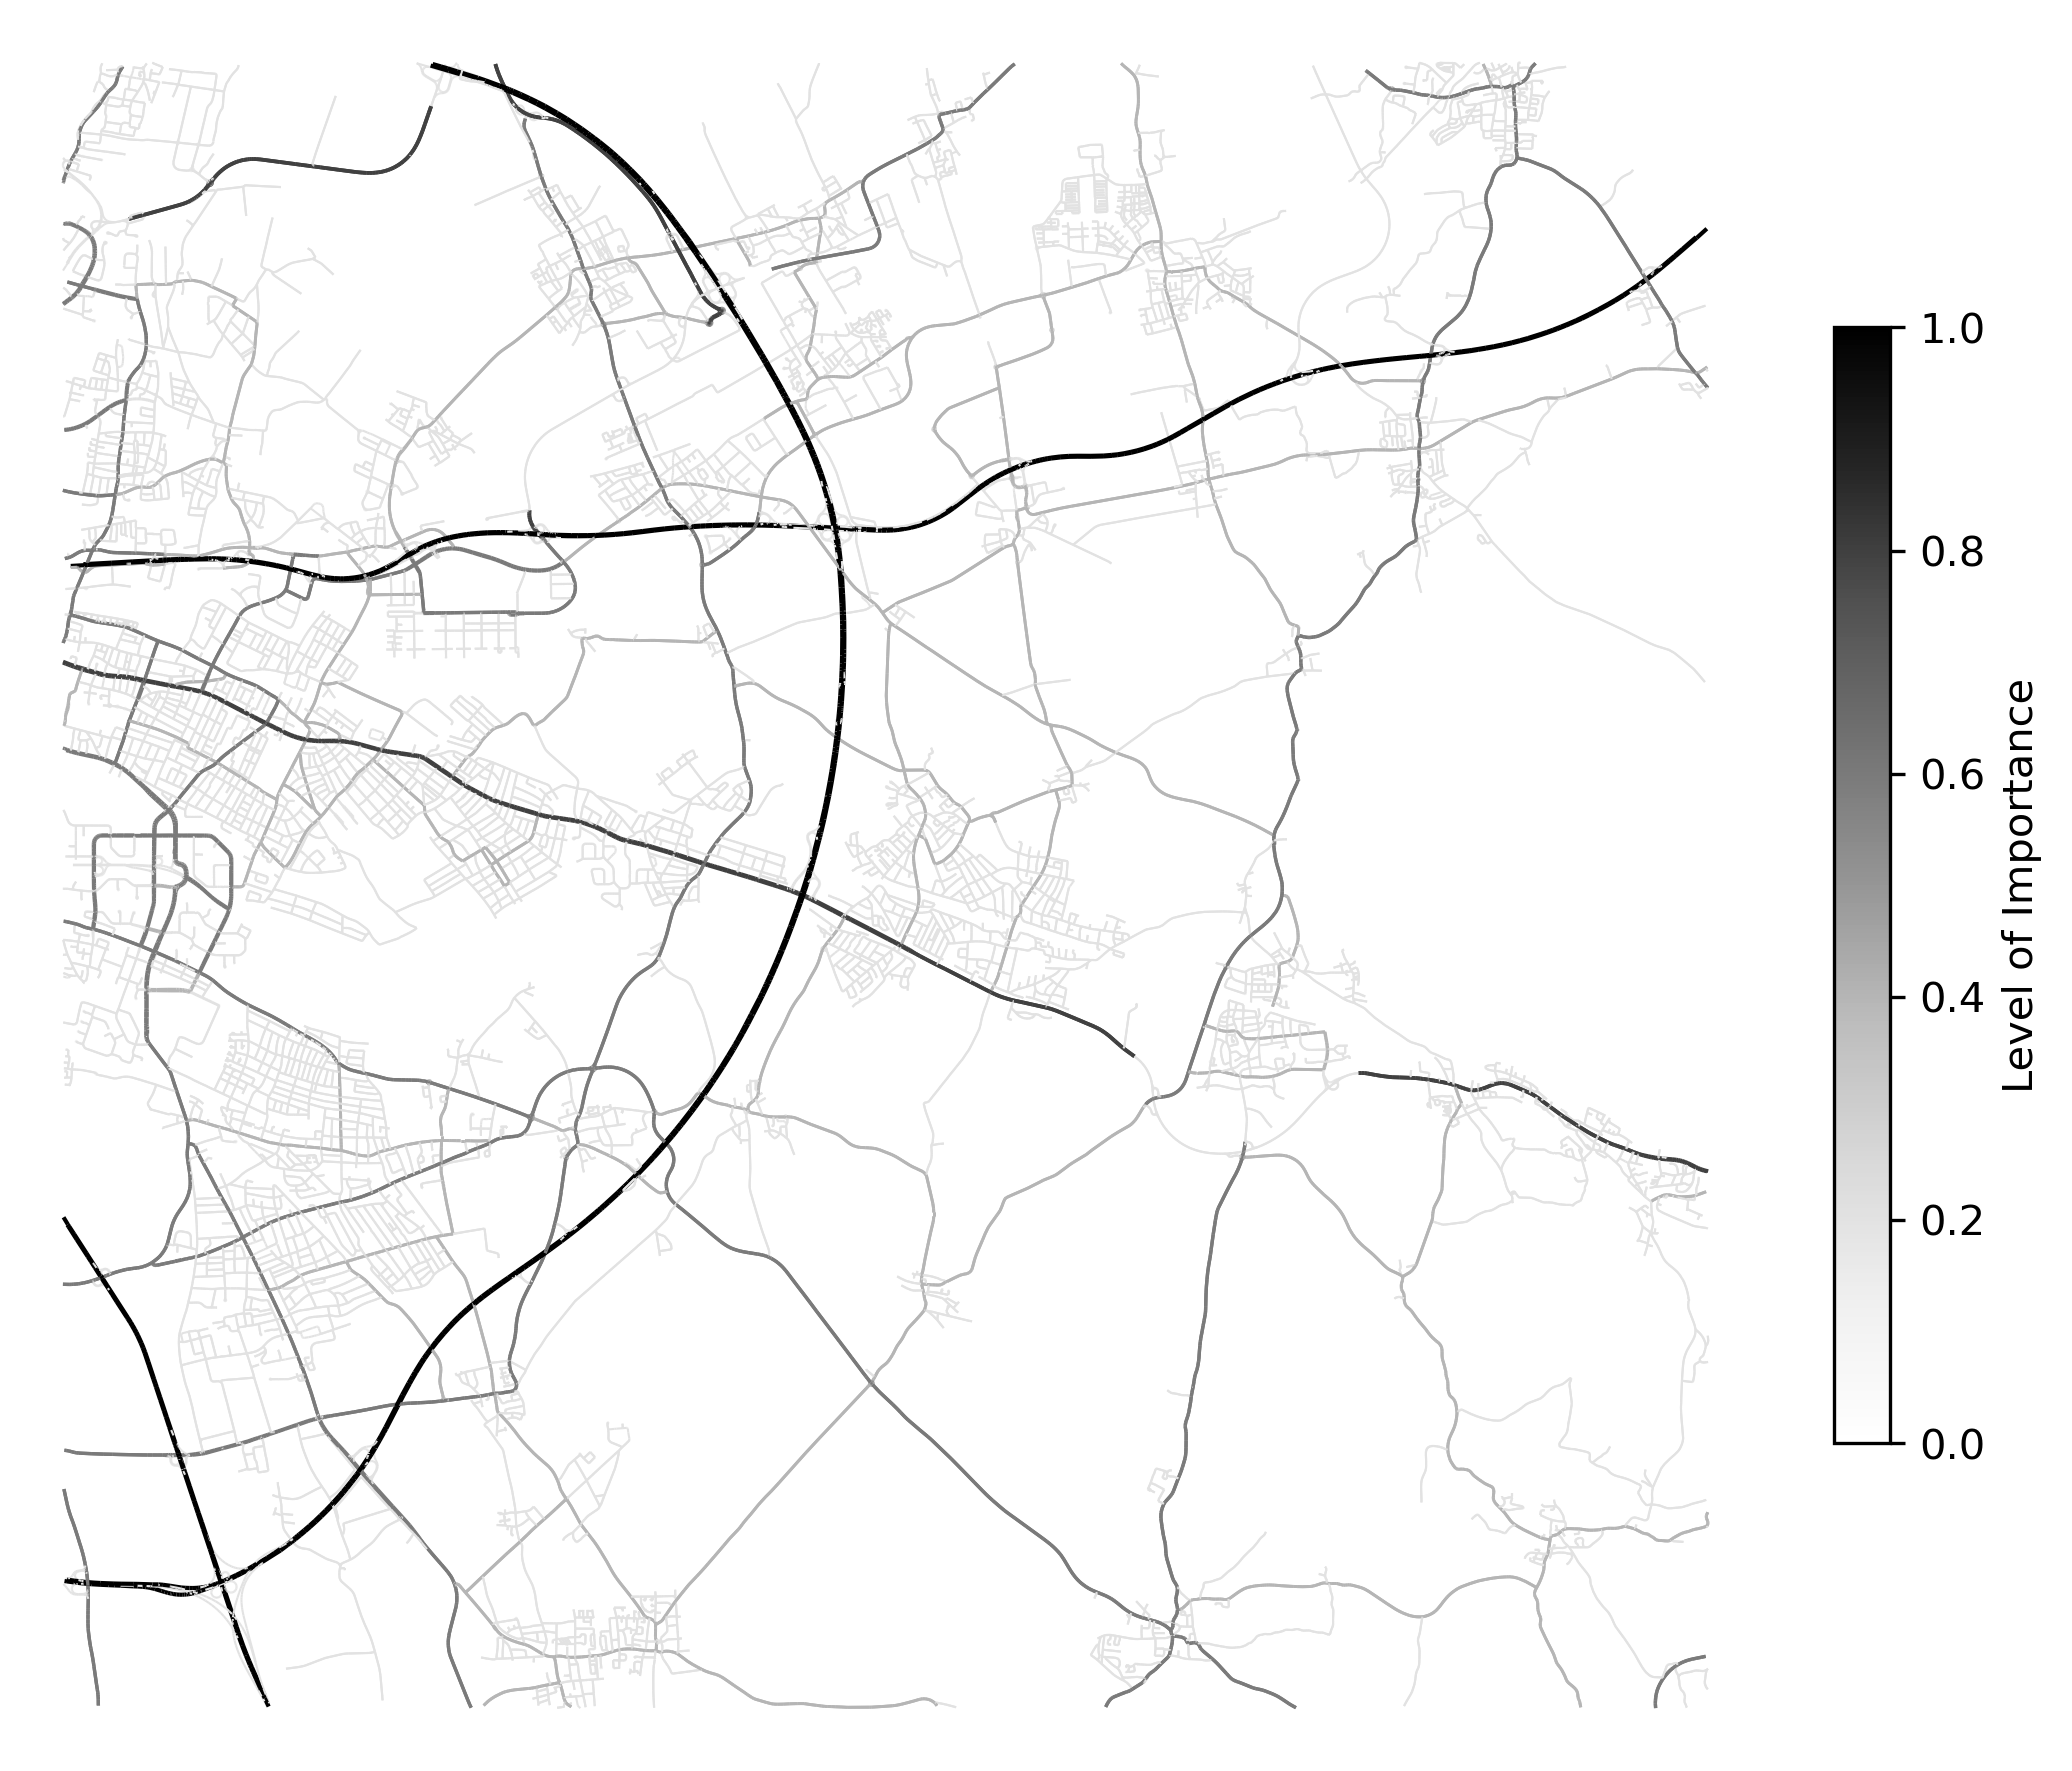
\includegraphics[width=0.5\textwidth]{figures/road_hierarchy.png}
    \caption[Hierarchie in Straßennetzen]{Hierarchie in Straßennetzen. Autobahnen (schwarz) sind
        ganz oben in der Hierarchie und sind sehr "`wichtig"'. Dagegen sind Straßen in
        Wohnsiedlungen weniger wichtig. \osmcr}
    \label{fig:road_hierarchy}
\end{figure}
Die Methode der Contraction Hierarchies nach Geisberger et al.
\cite{geisberger.workshop}~\cite{geisberger.thesis}~\cite{geisberger.exact} löst dieses Problem,
indem in einer Vorverarbeitungsphase Abkürzungskanten in den Graph eingefügt werden, die in der
Suche ausgenutzt werden. Die Abkürzungen erhalten dabei die kürzesten Wege \cite{Bast.20.04.2015}.
Während der Suche wird ein modifizieren bidirektioanlen Dijkstra-Algorithmus angewendet, der Kanten
die zu Knoten mit niedrigerem Level führen ignoriert. Dadurch wird der Suchraum extrem verkleinert,
was zu schnellen Antwortzeiten führt. Der CH-Algorithmus lässt sich in zwei Komponenten unterteilen:
\begin{enumerate}
    \item Vorverarbeitung: In dieser Phase werden die Knoten geordnet und die Hierarchie augebaut.
    \item Suche: Ausführung der bidirektionale Suche auf dem erweiterten Graph.
\end{enumerate}


\subsubsection{Vorverarbeitung}
In dieser Phase wird der Graph $G = (V,E)$ um zusätzliche Abkürzungskanten erweitert. Die
Abkürzungskanten werden im Prozess der Knotenkontraktion (eng. Node Contraction) eingefügt. Wenn ein
Knoten $v \in V$ \emph{kontraktiert} wird, dann wird er und alle Kanten die mit $v$ inzident sind
aus dem Graphen entfernt. Der Zeitpunkt des Entfernens ist gleichzeitig das \emph{Level} des
Knotens. Je später der Knoten entfernt wird, desto höher ist sein Level und damit seine Relevanz.
Wenn $v$ auf dem kürzesten Weg zwischen zwei benachbarten Knoten $u$ und $w$ liegt, dann wird eine
Abkürzungskante $e(u,w)$ mit $w(u,w) = w(u,v) + w(v,w)$ eingefügt, um den kürzesten Weg zu erhalten.

Abbildung~\ref{fig:ex_contraction} demonstriert den Prozess: Knoten $v$ soll kontraktiert werden und
damit er und seine inzidenten Kanten entfernt werden. Sei $U$ die Menge aller eingehenden Kanten und
$W$ die Menge aller ausgehenden Kanten, dann muss für jedes Paar überprüft werden, ob $v$ auf dem
kürzesten Weg <$u,v,w$> zwischen zwei benachbarten Knoten $u \in U$ mit $Level(u) > Level(v)$ und $w
    \in W$ mit $Level(w) > Level(v)$ liegt. Zum Beispiel ist dies zwischen $u_1$ und $w_2$ der Fall,
denn es gibt keine andere Möglichkeit $w_2$ zu erreichen, als über $v$. Um den kürzesten Weg zu
erhalten, wird eine Abkürzungskante $e(u_1,w_2)$ mit dem Gewicht
$w(u_1,w_2)=w(u_1,v)+w(v,w_2)=1+1=2$ eingefügt. Das gleiche gilt für <$u_2,v,w_1$> und
<$u_2,v,w_2$>. Der Weg von $u_1$ nach $w_1$ kann allerding über <$u_1,x,y,w_1$> schneller erreicht
werden (Kosten 3 sind kleiner als 4) und es muss daher keine Abkürzungskante eingefügt werden.
\begin{figure}[h]
    \centering
    \begin{subfigure}[b]{0.45\textwidth}
        \centering
        \begin{tikzpicture}
            \Vertex[x=0,y=0,label=v]{v}
            \Vertex[x=-2.5,y=1.5,label=$u_1$]{u1}
            \Vertex[x=-2.5,y=-1.5,label=$u_2$]{u2}
            \Vertex[x=-1,y=2,label=x]{x}
            \Vertex[x=1,y=2,label=y]{y}
            \Vertex[x=2.5,y=1.5,label=$w_1$]{w1}
            \Vertex[x=2.5,y=-1.5,label=$w_2$]{w2}
            \Edge[label=1](u1)(v)
            \Edge[label=1](u2)(v)
            \Edge[label=3](v)(w1)
            \Edge[label=1](v)(w2)
            \Edge[label=1](u1)(x)
            \Edge[label=1](x)(y)
            \Edge[label=1](y)(w1)
        \end{tikzpicture}
        \caption{Graph $G = (V,E)$}
    \end{subfigure}
    \begin{subfigure}[b]{0.45\textwidth}
        \centering
        \begin{tikzpicture}
            \SetVertexStyle[TextOpacity=0.2,FillColor=white,LineOpacity=0.2]
            \Vertex[x=0,y=0,label=v,opacity=0.2]{v}
            \SetVertexStyle[TextOpacity=1,FillColor=white,LineOpacity=1]
            \Vertex[x=-2.5,y=1.5,label=$u_1$]{u1}
            \Vertex[x=-2.5,y=-1.5,label=$u_2$]{u2}
            \Vertex[x=-1,y=2,label=x]{x}
            \Vertex[x=1,y=2,label=y]{y}
            \Vertex[x=2.5,y=1.5,label=$w_1$]{w1}
            \Vertex[x=2.5,y=-1.5,label=$w_2$]{w2}
            \SetEdgeStyle[TextOpacity=0.2,TextFillOpacity=0.2,Opacity=0.2]
            \Edge[label=1](u1)(v)
            \Edge[label=1](u2)(v)
            \Edge[label=3](v)(w1)
            \Edge[label=1](v)(w2)
            \SetEdgeStyle[TextOpacity=1,TextFillOpacity=1,Opacity=1]
            \Edge[label=1](u1)(x)
            \Edge[label=1](x)(y)
            \Edge[label=1](y)(w1)
            \Edge[fontsize=\large,label=2,color=red,bend=10,Direct,style=dashed,distance=0.3](u1)(w2)
            \Edge[fontsize=\large,label=4,color=red,bend=10,Direct,style=dashed,distance=0.3](u2)(w1)
            \Edge[fontsize=\large,label=2,color=red,bend=10,Direct,style=dashed](u2)(w2)
        \end{tikzpicture}
        \caption{Graph $G' = (V', E')$ mit $V' = V - \{v\}$}
    \end{subfigure}
    \caption[Knotenkontraktion]{Beispiel einer Knotenkontraktion}
    \label{fig:ex_contraction}
\end{figure}

Nachdem jeder Knoten kontraktiert wurde, erhält man einen neuen Graph  ${G^{*} = (V,E')}$, der als
\emph{Overlaygraphh} bezeichnet wird. $E'$ enthält alle ursprünglichen Kanten sowie die neu
hinzugefügten Abkürzungskanten (siehe Abbildung~\ref{fig:overlaygraph}).

Algorithmus zur Erstellung einer \ac{CH}

\begin{algorithm}[H]
    \caption{Highlevel-Algorithmus der Knotenkontraktion}
    \label{algo:contraction}
    \begin{algorithmic}
        \Function{Nodecontraction}{$G = (V,E)$}
        \ForEach{$v \in V$ geordnet nach Level}
        \ForEach{$(u,v) \in E$ mit $Level(u) > Level(v)$}
        \ForEach{$(v,w) \in E$ mit $Level(w) > Level(v)$}
        \If{<u,v,w> ist kürzester Weg von $u$ nach $w$}
        \State $E = E \cup \{e(u,w)\}$ mit Gewicht ${w(u,w) = w(u,v) + w(v,w)}$
        \EndIf
        \EndFor
        \EndFor
        \EndFor
        \EndFunction
    \end{algorithmic}
\end{algorithm}

\textbf{Beweis: Kontraktion erhält kürzeste Wege}
\begin{lemma}
    Sei $G = (V,E)$ ein beliebiger Graph und $G' = (V',E')$ der Graph nach Kontratkion von einem
    beliebigen Knoten $v \in V$ mit $V' = V - \{v\}$.\\
    Dann gilt für alle $s,t \in V'$: ${dist_{G'}(s,t) = dist_{G}(s,t)}$.
\end{lemma}
Lorem ipsum dolor sit amet, consectetur adipiscing elit. Sed euismod, nisl quis tincidunt
pellentesque, nunc nisl ultrices ipsum, quis aliquam nunc nisl ut nunc. Nulla facilisi. Nulla


\begin{figure}
    \centering
    \includestandalone[mode=buildnew]{tikz/figure_overlaygraph}
    \caption[Overlaygraph]{Overlaygraph nach Kontraktionsprozess. Der Graph $G^{*}$ enthält alle
        ursprünglichen Kanten sowie die neu hinzugefügten Abkürzungskanten.}
    \label{fig:overlaygraph}
\end{figure}

\subsubsection{Suche}